\documentclass[../main.tex]{subfiles}
\graphicspath{{\subfix{../img/}}}

\begin{document}

\section{Discussion} \label{sec:discussion}

\textit{Drosophila} is a well-established animal model for studying sleep due to its striking similarities in sleep regulation with vertebrates \parencite{shaferRegulationDrosophilaSleep2021,andreaniCircadianProgrammingEllipsoid2022}. R5 neurons have been reported to play an important role in sleep regulation in the fruit flies. Specifically, these neurons are thought to encode the homeostatic sleep drive in these animals \parencite{liuSleepDriveEncoded2016}. Similar to mammals,
\gls{swa} has been observed in \textit{Drosophila} brain during sleep and following sleep deprivation, and is believed to be generated at the level of the R5 neurons \parencite{raccugliaNetworkSpecificSynchronizationElectrical2019}. Furthermore, these neurons exhibit tonic spiking activity during the daytime, and bursting at night and after sleep deprivation \parencite{suarez-grimaltNeuralArchitectureSleep2021,liuSleepDriveEncoded2016}. 

Despite these observations, the cellular mechanisms underlying R5 neuronal activity remain poorly understood. Gaining insight into these mechanisms is crucial for a better understanding of the cellular basis of sleep regulation in \textit{Drosophila}.
In this study, conductance-based computational models were used to investigate the possible mechanisms responsible for several experimental findings related to the R5 activity.

First, electrophysiological studies in R5 neurons of \textit{Drosophila} have reported that their activity switches from tonic firing during the daytime to bursting during sleep and following sleep deprivation \parencite{liuSleepDriveEncoded2016,suarez-grimaltNeuralArchitectureSleep2021}. A study on gene expression in \textit{Drosophila} identified a negative correlation between increased sleep drive and the expression of a gene encoding a potassium channel known as \gls{eag} \parencite{doppSinglecellTranscriptomicsReveals2024}. Current thesis demonstrated that variation in the expression of the \gls{eag} channel could be a biologically plausible mechanism underlying the transition of R5 activity from bursting to tonic spiking, where the latter results from the reduction in the number of spikes per burst.

Second, an unpublished study by David Owald, Anatoli Ender, and colleagues reported existence of slow oscillations on the order of a few seconds following the blockade of $Na^+$ channels in Drosophila R5 neurons. These slow oscillations were hypothesized to be calcium spikes mediated by the T-type Ca$^{2+}$ channels. However, the results of the current study indicate that Ca$^{2+}$ channels alone cannot explain the observed slow-frequency ($<1$ Hz) oscillations due to their relatively fast kinetics. Therefore, other, or additional, mechanisms should be involved to account for the large interspike intervals.

Third, another unpublished study of David Owald, Anatoli Ender and colleagues showed, that knockdown of the T-type channels in R5 neurons causes increase in the minimal recorded membrane potential during bursting activity. Simulations showed that Ca$^{2+}$-activated $K^+$ channels could be the underlying mechanism behind this observation. It was demonstrated, that these channels can negatively modulate the minimal membrane potential when concentration of the T-type channels is reduced.


%%%%%%%%%%%%%%%%%%%%%%%%%%%%%%%%%%%%%%%
\subsection{Bursting and transition to tonic spiking}

It has been shown that compound \gls{swa} in \textit{Drosophila} R5 neurons results from the synchronized activity of single R5 neurons \parencite{raccugliaNetworkSpecificSynchronizationElectrical2019}. \gls{swa} itself has been associated with sleep need, quality and sensory gating during sleep \parencite{suarez-grimaltNeuralArchitectureSleep2021,raccugliaNetworkSpecificSynchronizationElectrical2019,gentThalamicDualControl2018}. R5 neurons start bursting and synchronize their activity with increasing sleep need \parencite{suarez-grimaltNeuralArchitectureSleep2021}. 
It has been reported that bursting can enhance the reliability of signal transmission by overcoming synaptic transmission failures, induce spikes more reliably in postsynaptic neurons, and influence synaptic plasticity more effectively in comparison to single spikes \parencite{lismanBurstsUnitNeural1997,kimBurstSynchronizationScalefree2019}.
Thus, the transition between spiking and bursting could potentially fascilitate synchronization of R5 neurons and, consequently, generation of the compound \gls{swa} in \textit{Drosophila} central complex. However, the cellular mechanisms underlying this change in firing pattern are not yet fully understood.

Transition between tonic spiking and bursting has been studied in various animal models, including mammalian thalamocortical neurons \parencite{wangMultipleDynamicalModes1994,suzukiTtypeCalciumChannels1989,vickstromTTypeCalciumChannels2020,liuMultipleConductancesCooperatively2008,mccormickModelElectrophysiologicalProperties1992}. Different mechanisms have been proposed to achieve both types of activity in the same cell.

The early work by Wang \parencite{wangMultipleDynamicalModes1994} proposed a model that exhibits bursting behaviour mediated by \gls{hcn} and T-type channels (see "T-type and \gls{hcn} channels" in Section \ref{subsubsec:ion_channel_contributions} for detalied description of corresponding bursting mechanism). In short, the \gls{hcn} and T-type channels form the slow subsystem, that first drives the membrane potential to the spiking threshold, and next to a hyperpolarized state. The strength of this drive depends on the magnitude of the hyperpolarizing external current: the stronger the hyperpolarizing current, the more \gls{hcn} channels activate and more T-type channels deinactivate (i.e. their inactivation gate opens). Apart from bursting, the model exhibits tonic spiking in two regimes. The first occurs when the hyperpolarizing current is too weak to fully activate the slow subsystem, resulting in a single spike. The Second occurs when the external current is depolarizing. In this case, the membrane potential is directly driven to the spiking threshold, resulting in tonic spiking at a frequency comparable to that within bursts.

However, the model proposed by Wang exhibits large variations in bursting frequency in response to small changes in the input current (see also Figure \ref{fig:rmp_models_phase}). Furthermore, the frequency of the tonic firing in R5 neurons is relatively low compared to the frequency of spikes within bursts (Figures \ref{fig:tmp_frequency_vs_zt} and \ref{fig:tmp_single_unit_r5_day_night}). Thus, the transition between tonic spiking and bursting in R5 neurons is less likely to be mediated by external input.

Bursting is defined as a slow alternating transition between spiking and steady states \parencite{rinzelFormalClassificationBursting1987}, while tonic spiking refers to the periodic firing of single spikes. By definition, if the number of spikes per burst is reduced to one, the activity becomes indistinguishable from tonic spiking. Thus, a change in the excitability of R5 neurons between day and night may result in reduction in the number of spikes per burst, underlying the observed shift in the activity patterns.

Several mechanisms have been proposed that reduce the number of spikes per burst, including upregulation of the A-type potassium channels, and downregulation of T- or L-type calcium channels \parencite{franciRobustTunableBursting2018,parkMathematicalModelSubthalamic2021}. Since potassium currents are hyperpolarizing, upregulation of the underlying channels opposes depolarization and can promote burst termination. Conversely, calcium currents are depolarizing, and downregulation of calcium channels may limit the ability to sustain bursting.

A recent study reported that expression of the gene encoding the potassium \gls{eag} channel negatively correlated with the increasing sleep drive \parencite{doppSinglecellTranscriptomicsReveals2024} in \textit{Drosophila} R5 neurons. Since R5 neuronal activity increases with elevated sleep drive \parencite{liuSleepDriveEncoded2016}, upregulation of the \gls{eag} channel in rested flies may contribute to early burst termination. Thus, the observed tonic spiking may result from a reduced number of spikes per burst, rather than from a fundamental change in the intrinsic response properties of R5 neurons.

Indeed, simulations showed that increasing the maximal conductance of the \gls{eag} channel can induce a transition from bursting to tonic spiking by the above-described mechanism. Bifurcation analysis revealed that this transition is mediated by the modulation of the $V$-nullcline in the fast (i.e. spiking) subsystem. Specifically, increasing the maximal conductance of the \gls{eag} channel alters the geometry of the $V$-nullcline such that the system spends less time in the spiking state - the region of the phase space where a stable limit cycle exists (Figure \ref{fig:spiking_to_bursting_wang_bifurcation}).

To investigate whether upregulation of the \gls{eag} channel could induce transition from bursting to tonic spiking, the parameters of the \gls{eag} channel were chosen such that its current does not significantly affect the bursting period. In the Wang model, this required a steep steady-state activation curve for the \gls{eag} channel, as the model exhibits large variations in bursting period with small changes in the external current (see also Figure \ref{fig:rmp_models_phase}). If the \gls{eag} channel is not fully deactivated during the interspike interval, it could effectively introduce an additional depolarizing current to the original Wang model (i.e., the model without the \gls{eag} channel) during the interspike interval, thus oppose depolarizing currents and, consequently, reduce the oscillation frequency, \textcolor{red}{as illustrated in Figure ...}.

\color{red}
By contrast, the Goldman model has been shown to be more robust to parameter variations and allows for more independent tuning of the spiking and resting states due to geometry of the nullclines of the corresponding system \parencite{franciRobustTunableBursting2018}.
This may explain why adding the \gls{eag} channel into the Goldman model required less parameter adjustment to achieve the desired effect. However, a more detailed analysis, such as aggregation of slow variables \parencite{franciModelingModulationNeuronal2014}, would be necessary to fully understand this behaviour.
\color{black}

The above-mentioned requirement not to modulate the oscillation period is a strict requirement with regard to the R5 neurons. As illustrated in Figure \ref{fig:tmp_single_unit_r5_day_night}, the frequency power spectra of R5 neurons have peaks at lower frequencies than $1$ Hz (bursting frequency at night). Thus, this shift could potentially also be attributed to the upregulation of \gls{eag} channels during the daytime, in addition to variations in synaptic input from other neurons.

% Interestingly, when many diffent types of channels are found in mammalian neurons, for some ion channels \textit{Drosophila} has only single gene for that channel. For example sodium channel (DMNaV) which accounts for both transient and persistent aspects of the current trace, T-type channels, slowpoke (?)... Thus, possible mechanisms of the transition is more constrained in \textit{Drosophila} than in mammalian species. However, it is worth to note, that the different channels can be generated not only via different genes, but there is also a mechanism called alternative splicing. Here, expression of single gene may result in construction of ion channels with slightly different properties (activation/inactivation kinetics) at the level of (translation ??? check, and define what translation is).

% Even if specific ion channel exists in \textit{Drosophila}, this is not sufficient condition for the transition between spiking and bursting. The expression of that ion channel should be different when the neuron exhibits spiking activity in comparison to when it bursts. One study showed ...

% EAG: different types (some has only activation, some does not, some are inactivated more by calcium, some not) - two papers on EAG

% Fast activation of EAG to terminate burst after first spike - generally not required. It is just thought that the R5 fires tonically. However, it can be that it fires only few (e.g. 2) spikes per burst. The model tells, that it can be possible to reduce the number of spikes to 1. However data analysis should be done to see what is in R5 neurons.

%%%%%%%%%%%%%%%%%%%%%%%%%%%%%%%%%%%%%%%
\subsection{What type of bursting behavior do R5 neurons exhibit?}

To my knowledge, the cellular mechanisms underlying bursting in R5 neurons have not been investigated. It remains unclear whether these neurons burst due to their intrinsic properties or if their bursting is driven by oscillatory input. Electrophysiological studies have suggested that slow-wave activity \gls{swa} may be generated at the level of R5 neurons \parencite{raccugliaNetworkSpecificSynchronizationElectrical2019}, which supports the hypothesis that their bursting arises intrinsically rather than being evoked by periodic external input.

As discussed in Section \ref{subsubsec:bio_burst_onset_offset}, neurons that exhibit bursting behaviour due to their intrinsic properties can be classified based on their response characteristics to the external input, and based on the cellular mechanisms that initiate and terminate bursts.

It has been shown that even for a fixed model structure (i.e. fixed set of ion channels, ion dynamics, etc.) variations in the maximal conductance of a single ion channel can lead to qualitatively different dynamical behaviours, even when the resulting voltage traces appear similar under baseline condition (i.e. prior to parameter variation) \parencite{alonsoVisualizationCurrentsNeural2019}.
Thus, multiple mechanisms could the observed firing pattern in R5 neurons.

As it will be discussed later, the proposed mechanisms for the transition of the activity between tonic spiking and bursting, and an increase in minimal recorded membrane potential following T-type channel knockdown, could, in principle, be generalized to all types of bursting models.


%%%%%%%%%%%%%%%%%%%%%%%%%%%%%%%%%%%%%%%
\subsection{Slow-freqeucny oscillations following $Na^{+}$ channel blockade}

The slow-frequency spiking with a period of several seconds has been observed following $Na^+$ channel blockade and is hypothesized to be mediated by T-type calcium channels.
Although these channels may be responsible for generating the spikes themselves, the long interspike intervals cannot be fully explained by the T-type current alone, given that the gating kinetics of these channels operate on a timescale of approximately $100$ ms \parencite{jeongCaa1TFlyTtype2015} \textcolor{red}{(see also Section ???)}.

A potential mechanism underlying the slow interspike interval could involve the activation of a depolarizing current with slow kinetics, which gradually drives the membrane potential toward the spiking threshold. Alternatively, it could arise from a slowly deactivating hyperpolarizing current, which delays the dominance of depolarizing currents and postpones spike initiation.

Regardless of the current type (hyperpolarizing, or depolarizing) and gating type (inactivating or non-inactivating),  the gating variables responsible for the slow interspike interval should evolve on a timescale of approximately one second at membrane potentials observed during the interspike interval. However, their kinetics must be significantly faster at more depolarized and/or hyperpolarized potentials in order to allow fast recovery during the brief duration of a spike ($\sim$$100$ ms, Figure \ref{fig:sleep_r5_knock_ttx_voltage}).

In the context of the first-order kinetic gating models (when activation and inactivation gates have only two - open and closed states), this implies a steep voltage dependence of the gating time constant $\tau(V)$ (see Equation \ref{eq:differential_gating_steadyst_timeconst}). 
Specifically, it must vary by an order of magnitude within a relatively narrow voltage range ($15$-$20$ mV), corresponding to the difference between the membrane potentials at the spike peak and at steady state (Figure \ref{fig:sleep_r5_knock_ttx_voltage}).

Alternatively, the kinetics may be modelled using higher-order kinetic schemes. These models account for gating mechanisms involving more than two states, including multiple closed or inactivated states and distinct transition pathways between them. Such models are commonly implemented using Markov chains \parencite{mangoldIdentificationStructuresIon2021}. For example, the model proposed by \textcite{wangModelTtypeCalcium1991} for the T-type calcium channel includes one open and two closed states in the inactivation gate of the channel, thereby capturing more complex gating dynamics than a first-order kinetic model.

Another mechanism, that to my knowledge has not been reported in the literature, may involve the interplay between calcium- and voltage-gated potassium channels (such as the large-conductance BK channel), voltage-gated calcium channels (e.g., T- or L-type), and intracellular calcium dynamics.
Similar to the previously described mechanism, slow deactivation of potassium channels could lead to a gradual dominance of depolarizing currents, eventually driving the membrane potential toward the spiking threshold.

Which mechanisms might underlie the prolonged deactivation of the BK channels?
Full activation of BK channels requires both - an increase in intracellular calcium concentration and sufficient membrane depolarization \parencite{liuMultipleConductancesCooperatively2008}.
While many modelling studies assume rapid calcium decay, typically ranging between $1$-$13$ ms \parencite{huguenardSimulationCurrentsInvolved1992,golombContributionPersistentNa2006,parkMathematicalModelSubthalamic2021}, experimental studies have reported two distinct timescales of calcium decay, a fast ($10$ms) and with a slow component on the order of hundreds of milliseconds \parencite{theisBenchmarkingSpikeRate2016,koesterCalciumDynamicsAssociated2000}.

Moreover, calcium channels may continue to mediate inward currents at membrane potentials observed during the interspike interval. Taken all together, I suggest the following scenario: the initial rapid hyperpolarization during a spike could be mediated by BK channels, whose activity is supported by both depolarization and the rise in intracellular calcium following the spike onset. At hyperpolarized potentials, BK channels begin to inactivate due to voltage sensitivity and/or the fast component of the calcium decay. However, if the activation gate of BK channels remains partially open near the resting potential, they could undergo slow deactivation driven by the slow component of calcium decay.

Combining these altogether, if the initial fast hyperpolarization could be mediated by the BK channels, the first, fast decay in the membrane potential during spike can be mediated by the BK channels that inactivate due to their voltage dependence and the fast component of the calcium decay. However, if the activation gate of these channels is open in the membrane potentials where the neuron exhibits almost steady state, they can be slowly deactivated by the slow component of the calcium removal. This deactivation might be further slowed down by the current mediated by the calcium channels. Thus, a combination of the slow timescale of the calcium decay, together with calcium influx during steady state, could explain the large oscillation periods between the observed spikes.

This deactivation may be prolonged by continuous calcium influx through T- or L-type calcium channels active at subthreshold potentials. Thus, continuous calcium entry, together with deactivation of BK channels via the slow component of calcium decay, could explain the long interspike intervals in the R5 neurons following blockade of sodium channels.

Lastly, the presence of oscillations after blockade of sodium channels does not exclude the possibility that the neuron receives input from other sources, such as electrical coupling via gap junctions, or interactions with astrocytes, rather than through conventional synaptic transmission.

The mechanism responsible for generating slow oscillations in R5 neurons following sodium channel blockade, as well as the potential involvement of external sources, remains unknown. Further experimental studies are needed to investigate this observation.


%%%%%%%%%%%%%%%%%%%%%%%%%%%%%%%%%%%%%%%
\subsection{Increase in resting membrane potential following T-type channel knockdown}

\color{red}

This was quite interesting finding as to my knowledge such effect of t-type knockdown on minimal membrane potential has not been reported before. Actually, quite the contrary has been reported (cite). 
One of the modeling studies illustrated that in specific parameter ranges the model that they had could result in increase of minimal membrane potential in relatively narrow range (approx, 80\% blockade). Noteworthy, this study did not concentrate on this behavior at all. It is just one of their plots showed that. Because the dynamics are strongly affected by parameters and there are many many parameters, the results of the computational studies cannot guartee that such effect is not plausible. First, one needs to find specific parameter regime. Second, one should concentrate on specific detail. It can be the case, that some of the models has this effect, but it was just not reported.

And this contrary is the intuitive one. Since calcium is depolarizing current, removing it should be expected. This might suggest calium dependent process.

This does not necessarily imply that the bursting has to be stopped by KCa channels. Theoretically, similar effect should be observed regardless of the bursting mechanism. However, more work should be done to investigate this and can be one of the goals of the future work.

\color{black}

% RMP depolarized following SD (Connection to T-Type channels and increased RMP in knockdown.
%     Effect of affector circuits following SD, as Ca gated K channels should have the opposite effect ???)
%     \parencite{liuSleepDriveEncoded2016}


%%%%%%%%%%%%%%%%%%%%%%%%%%%%%%%%%%%%%%%
\subsection{Limitations of current approach}

These have been identified, but still needs to be put together to construct one model. It is unknown whether such parameter set exist for ion channel + calcium dynamics, or some other aspects should be modelled? Like multiple compartment??? Or maybe other mechanisms, such as calcium dependent synaptic plasticiy is required? Or modulation of other channels besides EAG?

T-Type ca channels are located at presynaptic terminals. What is the consequence?

\parencite{blumAstroglialCalciumSignaling2021}: astrocytes and Toll receptors on R5 neurons.
    Toll might trigger gene expression (??? Need a bit more literature research)

Single compartment

Calcium release in cytosole

Although it was not investigated in this thesis because of the limited amount of time, the proposed mechanisms of transition between spiking and bursting, as well as increase in minimal membrane potential following T-type channel blockade should not in general depend on type of bursting (intrinsic vs forced, tonic vs inhibition-rebound).
Wang - interplay between h and T-type, Goldman - termination by KCa.

Cannot explain if T-type channels mediate for bursting

%%%%%%%%%%%%%%%%%%%%%%%%%%%%%%%%%%%%%%%


%%%%%%%%%%%%%%%%%%%%%%%%%%%%%%%%%%%%%%%
\subsection{Considerations for modeling R5 neurons}

\begin{itemize}
    \item In conntrast to three-compartment mmodel, single-compartment model could only estimate either I-V relationship, or LTS, but not both,
    with LTS observed in case of increased maximal conductance of T-Type channels. \parencite{destexheDendriticLowthresholdCalcium1998}
\end{itemize}

Furthermore, for simplicity, single compartment conductance based model was chosen.
Such model 1) does not account for dendritic computations, and 2) assumes uniform distribution of
ion channels. \textcolor{green}{Nonlinear interactions in the multi-compartment model might better explain
the experimental results without need of L-Type Ca$^{2+}$ currents.}

Single and three compartment neuron model - Destexhe \parencite{destexheDendriticLowthresholdCalcium1998}.

Different models
\begin{itemize}
    \item Ion channels
    \item Same model, different parameter regimes
    \item If not mediated by t-type, they do not include T-Type channels
    \item Different goals: inhibition rebound vs induced bursting
    \item Slow variable for calcium oscillations
    \item Misreported parameters (HM neuron in paper and in one thesis)
\end{itemize}

Tuning the parameters of conductance based model to produce specific dynamical characteristic is a hard problem. First, due to large number of parameters, investigating every parameter combination even in the constrained parameter space is computationally inefficient. Second, predicting the effects of an arbitrary parameter perturbation on the solution is challenging and largely unresolved problem \cite{alonsoVisualizationCurrentsNeural2019}. Several approaches have been proposed to find parameters reproducing the desired dynamics. Prinz and colleagues constructed a database of 1.7 million single-compartment neurons by individually varying $8$ maximal conductances for one particular model of choice \parencite{prinzAlternativeHandTuningConductanceBased2003}. Others proposed using evolutionary algorythms to find set of parameter combinations leading to similar voltage responses in model neurons \cite{alonsoVisualizationCurrentsNeural2019}. It has been demonstrated that such multiple parameter combinations can result in qualitatively same membrane potential dynamics, even within the same single-compartment model \cite{alonsoVisualizationCurrentsNeural2019}.

Neurons differ by expression of ion channels, location of ion channels, concentrations. Thus,
different models incorporate different ion channels and max conductances depending on neuron of interest

It is hard to fit generally, as the ion channel dynamics overlap - e.g. extending time constant
might affect other currents and fitting might be the best method

Thing to fit the neurons (blue thing, find what it was)

Different effects with changing one variable also is observed when two parameters are varied (my plot) :D Now you can imagine what will happen in higher dimensions :D

\begin{figure}[!t]
    \centering
    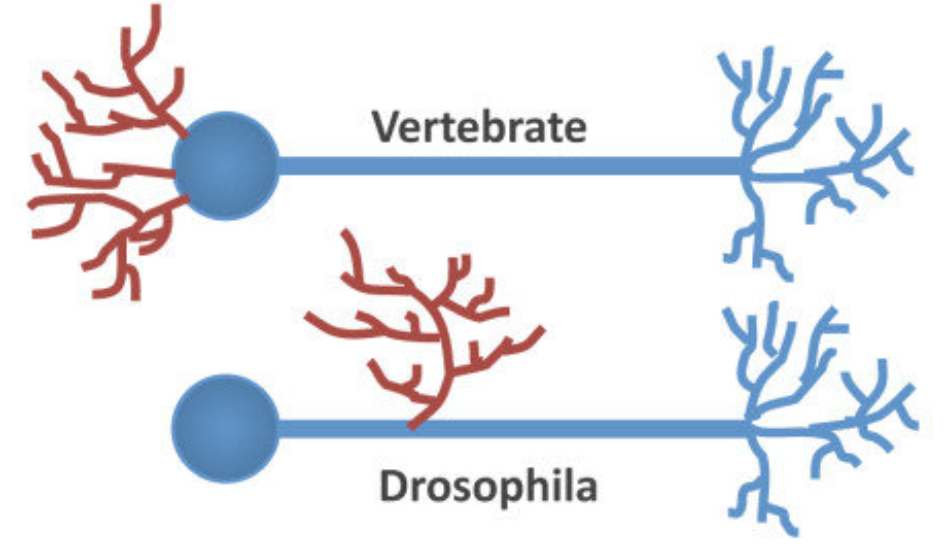
\includegraphics[width=0.55\linewidth]{../img/modeling_r5/examples/drosophila_neuron_morphology.png}
    \caption[Neuron morphology in \textit{Drosophila} and Vertebrates]{
        \textbf{Comparison of neuron morphology in \textit{Drosophila} and Vertebrates.}
        In comparison to vertebrates,
        the neurons in \textit{Drosophila} have unipolar morphology. Therefore synaptic potentials
        travelling from the dendrites (red) to spike initiation zone bypass cell body
        (blue circle). Figure adapted from \parencite{spindlerBazookaMediatesSecondary2011}.
    }
    \label{fig:morphology_drosphila_vs_mammalian}
\end{figure}

Although R5 neurons share similar functional characteristits with thalamic neurons,
morphology of neurons in \textit{Drosophila} is significantly different from those in vertebrates
\ref{fig:morphology_drosphila_vs_mammalian}. 
Unlike vertebrates, \textit{Drosophila} neurons have unipolar morphology. Because of this morphology,
synaptic potentials travelling from dendrites to spike initiation zone bypass cell body.
Because of this morphology, the cell body of \textit{Drosophila} neurons is
electronically segregated from other cell regions, suggesting that it is not involved
in synaptic integration \parencite{gouwensSignalPropagationDrosophila2009,tuthillLessonsCompartmentalModel2009}.
Furthermore, it has been found that, in contrast to vertebrates, dendrites of
\textit{Drosophila} neurons (slecifically, \gls{kc}) are not solely postsynaptic, but
also form presynaptic active zones \parencite{christiansenPresynapsesKenyonCell2011}.

Multcompartment: increases robustness to parameter variations

Same model could exhibit different type of bursting in relation to external current (tonic, inhibition-rebound...) depending on parameter regime \parencite{parkMathematicalModelSubthalamic2021}.

%%%%%%%%%%%%%%%%%%%%%%%%%%%%%%%%%%%%%%%


Did not incorporate calcium in day/night - calcium activates k dependent K channels + effectively modulates calcium channel strength -> Thus the effect might be even better

Calcium is important in cellular processes (liu)

KCa channel may be important and calcium can be important here as well

EAG channel may be important

Although for many bursting neurons H current is necessary (blocking of H current blabla, find literature)
it is not mandatory for \gls{ahp} (image from Izhikevich book and models that have ahp but still
have very nice bursts or ahp).

T-type modelling - GHK model might be better :))))))

\subsection{Summary and outlook}

EAG is potential mechanism, we need something else for slow oscillations, calcium dependent potassium channel may contribute.

Number of spikes per burst, burst width, ...

It is not known how R5 neurons burst. However, the proposed mechanisms are potentially not constrained to a single bursting model and potentially could be generalized to other bursting mechanisms.

Width of the burst? Slow oscillations? Synchronisation and how eag affects it? Increase in synchronization with TUBU? Helicon cells and R5 - filtering viual information? dFSB fascilitating sleep via inhibition of helicon cells?

\parencite{krummSlowlyOscillatingBrain2021} implemented R5 and helicon cells based
on Izhikevich model of burstin neurons \parencite{izhikevichSimpleModelSpiking2003}.

\parencite{krummSlowlyOscillatingBrain2021} suggested the inhibitory synapses between R5 and
helicon cells to explain this observation.


Blocking NMDR - irregular interburst interval, controls - regular.
    Chaos??? (further support for square-wave)
    \parencite{raccugliaNetworkSpecificSynchronizationElectrical2019,izhikevichNEURALEXCITABILITYSPIKING2000}


Nonlinearities and opposite effects: such parameter range have been found in the investigated models as well, but was not analyzed within the scope of this thesis. Are these regions model or parameter/range specific? To what extent?

EAG - transition between spiking and resting, dFSB - increased oscillatory power following SD

EAG - and shift of the power spectra peak (oscillation freuqnecy) to lower values

Slow oscillation - modeling

\color{red}

% ------------------------------
% IMPORTANT!!!:
% \begin{itemize}
%     \item Citations from Lauras thesis
%     \begin{itemize}
%         \item In the Down state, Helicon is entrained to R5's compound rhythmicity via excitatory
%         coupling. This leads to a relatively short offset (7 ms) between the two signals
%         \item For Helicon in the Down state, we find a much larger and negative offset of 
%         -77 ms (fig. 2.34a). We assume this is because Helicon now also receives inhibitory inputs
%         from R5 neurons which prevent Helicon from firing and therefore lead to a small anti-phase
%         correlation between the two signals.
%     \end{itemize}
%     \item From Manuscript:
%     \begin{itemize}
%         \item (Simulations). This is also in line with our experimental data, which show
%         that the balance controls the degree of synchronization between excitatory and inhibitory
%         drive and determines whether the networks are in the shifted or synchronized configuration
%     \end{itemize}
%     \item Remarks
%     \begin{itemize}
%         \item In the Lauras thesis, in the second note it should be written "Up State" instead of
%         "Down State". However, this state
%         corresponds to daytime rather than night. Thus this will not explain the experimental
%         observations (shifted state at night)
%         \item In manuscript, 1) there is no inhibition from R5 to helicon at night. Thus,
%         the temporal shift might be due to the synaptic time constant between helicon and R5,
%         rather than interplay between excitation and inhibition between R5 and Helicon.
%         Synaptic time constant was set to be 100 ms (similar to resulted time delay between helicon and R5).
%         Thus, when additional input was provided to helicon, here helicon might drive R5 and R5 might burst due to intrinsic properties.
%     \end{itemize}
% \end{itemize}

% \color{black}


% \noindent\hrulefill

% \color{orange}

% Facts:
% \begin{itemize}
%     \item Ca1T-null mutants showed increased sleep \parencite{jeongCaa1TFlyTtype2015}
%     \item Ca1T in drosophila are located at presynaptic terminals of R5
    
% \end{itemize}

% \color{red}

% Discussion:
% \begin{itemize}
    
    
    

    % \parencite{jeongCaa1TFlyTtype2015} Flies lacking T-Type channels increase amount of sleep. If bursting in
    % R5 requires sleep, than this is on the one hand counterintuitive result. Although, knocking down
    % expression of T-Type channels in whole fly might have more complex effects on sleep, as other
    % circuits that affect R5 acitivty also will lack the similar channel that might result in this
    % observation.

    

    % BRP - Important for regulation of calcium channels (???)

    % \item Raccuglia: frequency of R5 activation and locomotion. Actitation was done by optogenetics. If bursting is
    % mediated by hyperpolarization activated current, then it can be that optogeneetically one directly
    % activates fast system. Thus, you will need specific frequency of activation to induce similar
    % effect (intrinsic bursting 1Hz).

    % \item Other mechanisms are likely to be involved during normal, undisturbed sleep \parencite{liuSleepDriveEncoded2016}.
    
    % \item Manuscript: "Because R5 activation can also entrain
    % dFSB activity during the day (Extended Data Fig. 2a-c), we suspect that this interaction would
    % effectively set helicon cells to the downstate (night setting), allowing for entrainment of
    % helicon by R5."
    % \begin{itemize}
    %     \item This can also be due to DN1p clock neurons, not through dFSB
    %     \item While helicon cells can be set to the downstate through DN1p-dFSB circuit,
    %     the SWA could be achieved through R5-helicon-dFSB circuit, where
    %     excitatory synapses from helicon drive SWA in dFSB. It will be interesting
    %     to see the time lag correlation between dFSB-helicon and dFSB-R5 in the SD condition.
    %     Or even better - granger causality (as correlation does not tell us about causality).
    %     (Paper for method: 
    %     Reassessing hierarchical correspondences between brain and deep networks through direct interface
    %     \url{https://www.science.org/doi/10.1126/sciadv.abm2219})
    % \end{itemize}

% \end{itemize}

% \color{black}


    

%% Not ture :)))
% Notably, out of the identified sleep-pressure-inducing neurons, only the inactivation of R5 neurons had effect on
% rebound sleep,  while inactivation of other neurons had no effect. \textcolor{red}{\textbf{(This can be related to the Raccuglia 2019 - reduced neurotransmitter release
% might affect R5 synchronization. Interesting question: as excitatory drive is important for synchronization,
% what will happen if only inhibitory synapses are blocked? No reduction in rebound sleep?)}}


% We assume that the R5 neurons are intrinsic bursters, i.e. they can exhibit bursting activity due to
% cell-autonomous conductances, even in case of constant input current.
% Thus, when concentrating on simulations of R5 neurons to study either transition between
% bursting and tonic spiking or effects of blocking specific ion channels, external input to R5 neuron
% is modelled as a constant.

% \begin{itemize}
%     \item Turrigiano et al 1995 \& Tang: \url{https://pmc.ncbi.nlm.nih.gov/articles/PMC6578228/pdf/jneuro_15_5_3640.pdf}
%     \item Fazli et al 2020, Bertram et al 2000: phantom bursting + no sodium
% \end{itemize}



Do the simulations with noninstantaneous activation for Wang model - maybe the transition between
spiking and resting will be easier

Maybe try to hand-tune one TTX oscillation and then use optimisation to fit others

Slow oscillations in small parameter region - input current is important, as it only affects the V-nullcline. You change it, you move away - you move away from the slow manifold if the trajectory passes along it.

switching from day to night will not depend on type of bursting


% \item The sharp transient at the end of the pulse in recordings (Fig. \ref{fig:i_v_relationship_jeong})
% is most likely due to passive membrane properties. The membrane time constant of R5 neuons is not known.
% Arbitrarily incorporating $\tau=10$ms time constant reproduced the sharp transient (not shown here).
% However 1) as Drosophila T-Type channels were expressed in frogs (Oocites), fitting membrane time constant
% will not be helpful in modeling Drosophila R5 neurons; 2) The passive membrane time constant

% \begin{itemize}
%     \item Estimated number of activation gates for Drosophila T-Type ion channels is 3.
%     \item modeling the ion channel using Ohmic relationship between current and voltage
%     did not procude good fits to observed current-voltage (I-V) relationship.
%     \item The current-voltage relationship was reproduced when
%     Goldman-Hodgkin-Katz (GHK) voltage flux equation was used instead of Ohmic current
%     \item GHK equation models explicit relationship between current, voltage, temperature and
%     intra-/extracellular ion concentrations.
%     \item The fit of simulated I-V relatoinship to the observed data was improved when
%     the steady-state activation function was shifted along $V$ axis,
%     and corresponding time constant was scaled and shifted along $V$ axis (parameters for
%     shifting and scaling were taken to be free parameters during optimization)
% \end{itemize}

\end{document}